\documentclass[a4, 12pt]{article}

\usepackage[margin = 2cm]{geometry}
\usepackage{graphicx}
\usepackage{caption}
\usepackage{subcaption}
\usepackage{float}
\usepackage{hyperref}
\setcounter{secnumdepth}{0}

\usepackage{amsmath}
\usepackage{amssymb}
\usepackage{siunitx}
\usepackage{tcolorbox}
\usepackage{xcolor}
\usepackage{listings}

\definecolor{dkgreen}{rgb}{0,0.6,0}
\definecolor{gray}{rgb}{0.5,0.5,0.5}
\definecolor{mauve}{rgb}{0.58,0,0.82}
\lstset{frame=tb,
  language=c++,
  aboveskip=3mm,
  belowskip=3mm,
  showstringspaces=false,
  columns=flexible,
  basicstyle={\small\ttfamily},
  numbers=none,
  numberstyle=\tiny\color{gray},
  keywordstyle=\color{blue},
  commentstyle=\color{dkgreen},
  stringstyle=\color{mauve},
  breaklines=true,
  breakatwhitespace=true,
  tabsize=3
}



\title{Measuring Climate Trends using ROOT}
\author{MNXB01 \\ Philip J. Fredholm \\Lee Chun Hin }



\begin{document}
\maketitle
\tableofcontents
\newpage

\section{Introduction}
In order to be able to draw conclusions about some physical phenomena, such as the climate of Earth, it is sometimes necessary to be able to process large amounts of data. In order to save a considerable amount of time doing so, it is often the case that such processing may be done with the help of a computer programming language. The purpose of the subject of this report has been to try to use the programming language C++ in order to to process data from the SMHI OpenData initiative and draw conclusion about climate and weather trends from this data. In particular, attempts have been made in order to analyse the data and find the distribution of coldest and hottest day of each year, the first day of summer as well as to analyse the temperature of a given day of the year (August 23rd) over many years.

\section{Theory}
\section{Method}
\section{Results}


%Philip's Figures
\begin{figure}[H]
\centering
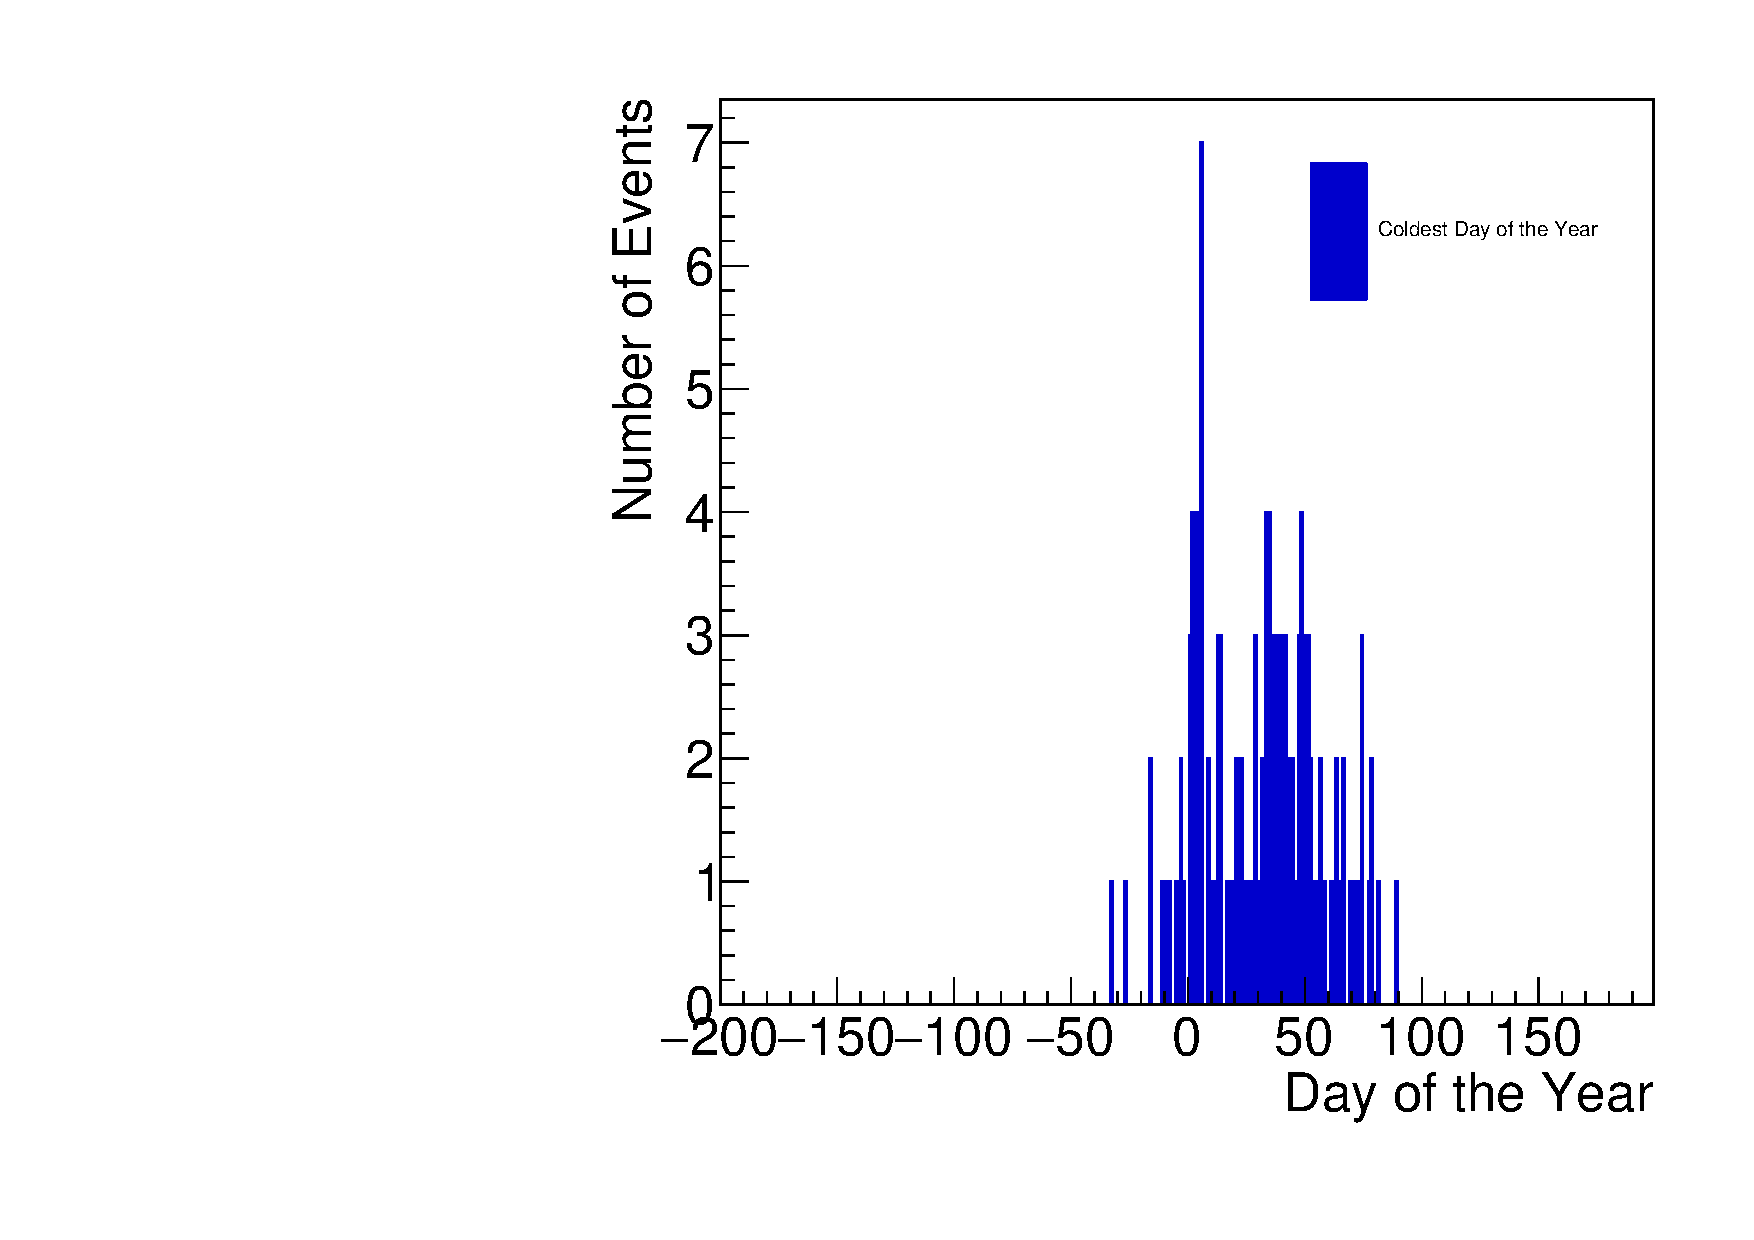
\includegraphics[scale=0.50]{philipCold.pdf}
\caption{Shows the number of occurrences of a specific day being the coldest day of that year in Borås. Negative days indicate that the day was in the end of the previous year.}
\end{figure}


\begin{figure}[H]
\centering
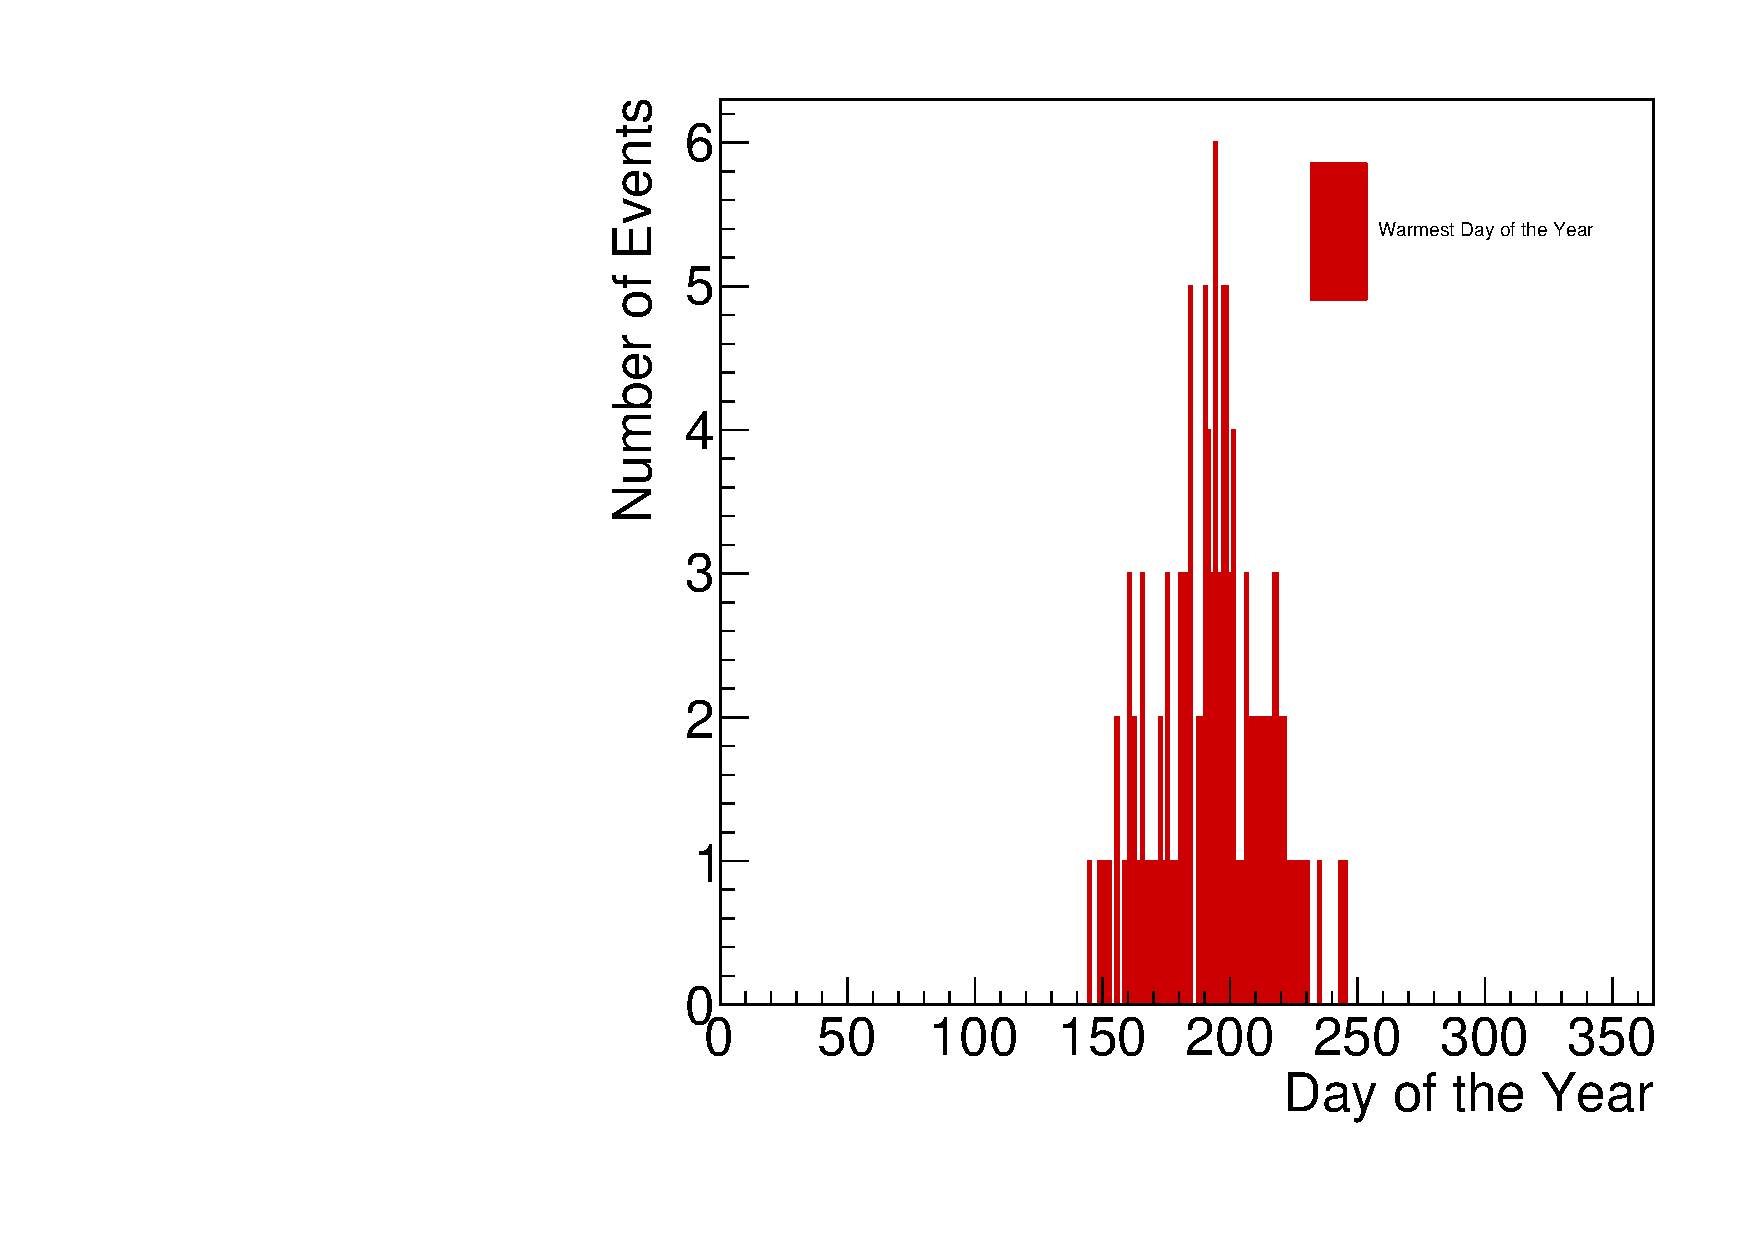
\includegraphics[scale=0.50]{philipHot.pdf}
\caption{Shows the number of occurrences of a specific day being the warmest day of that year in Borås.}
\end{figure}

\begin{figure}[H]
\centering
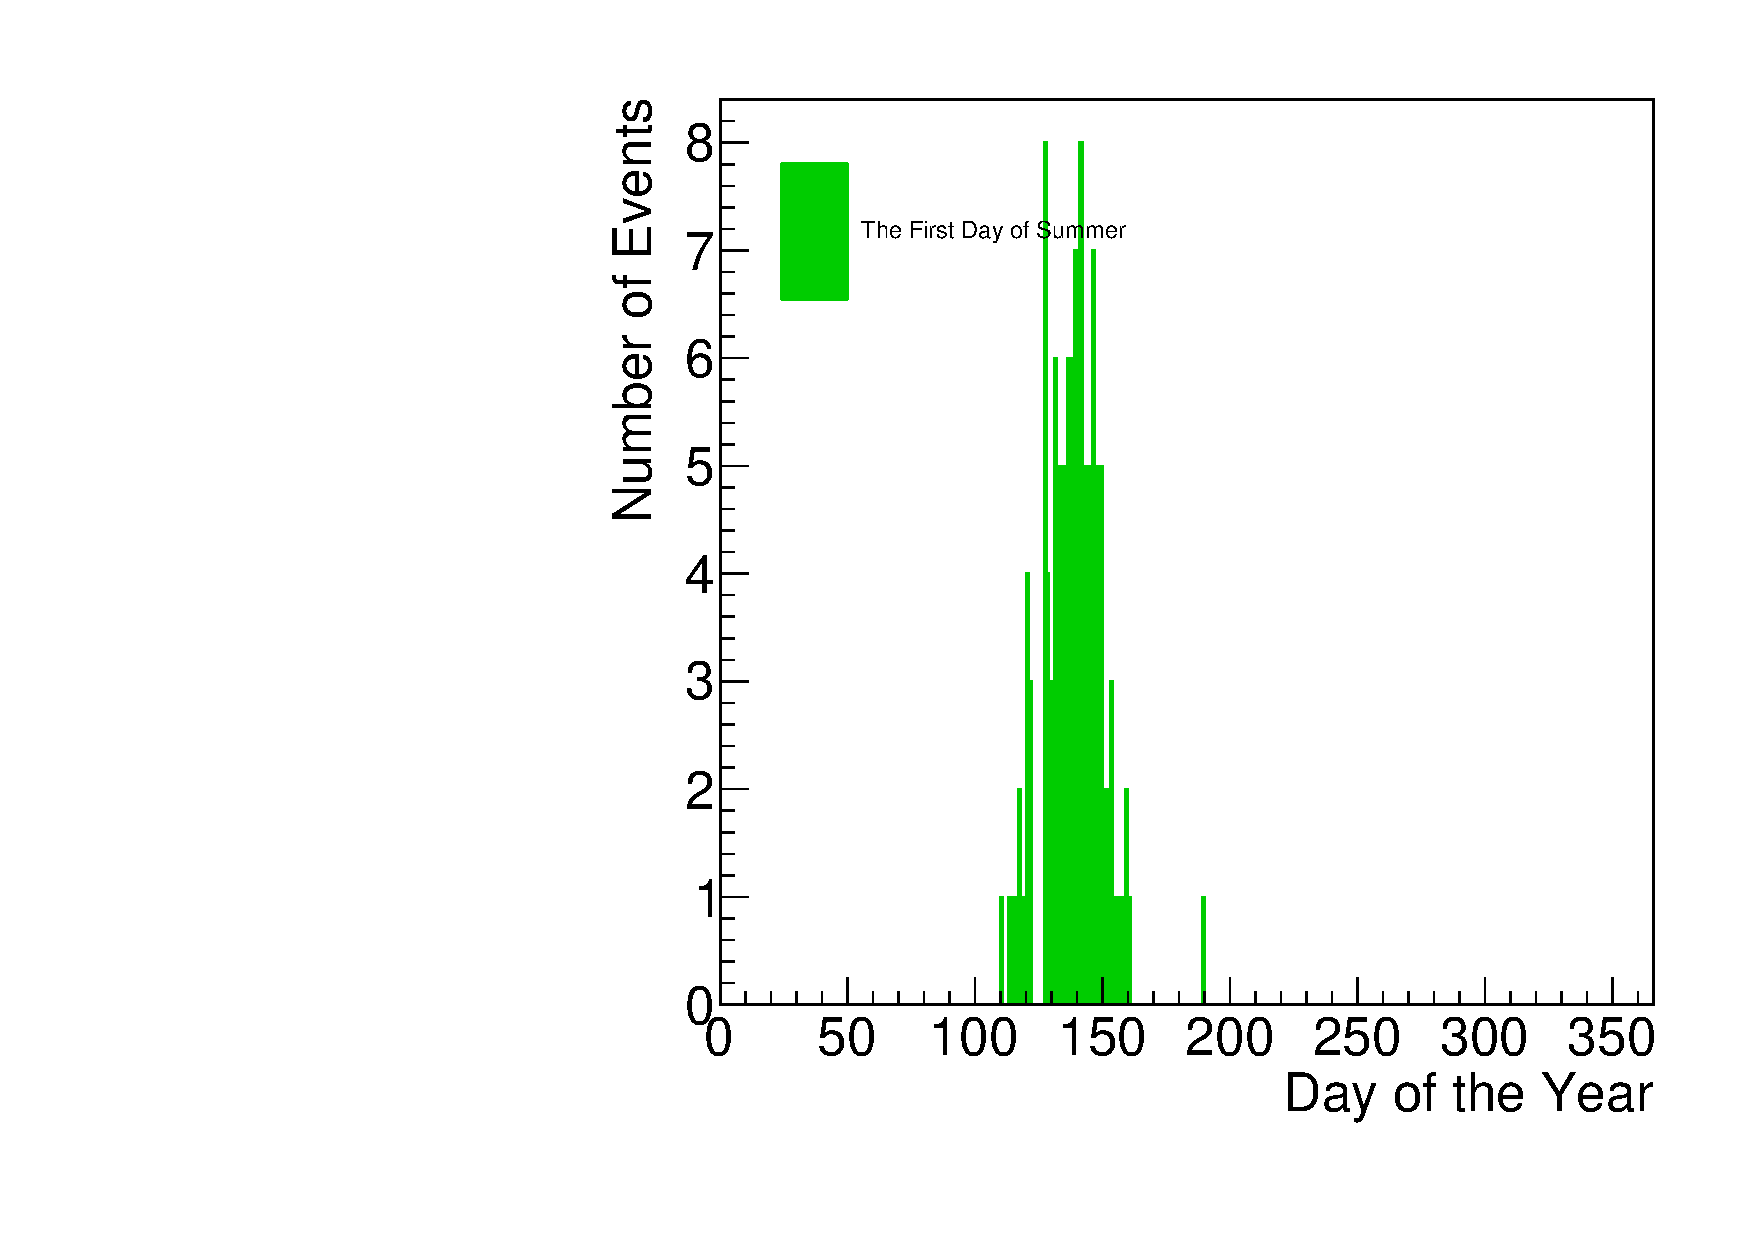
\includegraphics[scale=0.50]{philipSummer.pdf}
\caption{Shows the number of occurrences of a specific day being the first day of summer that year in Borås.}
\end{figure}
\newpage




%Chris's Figures
\begin{figure}[H]
\centering
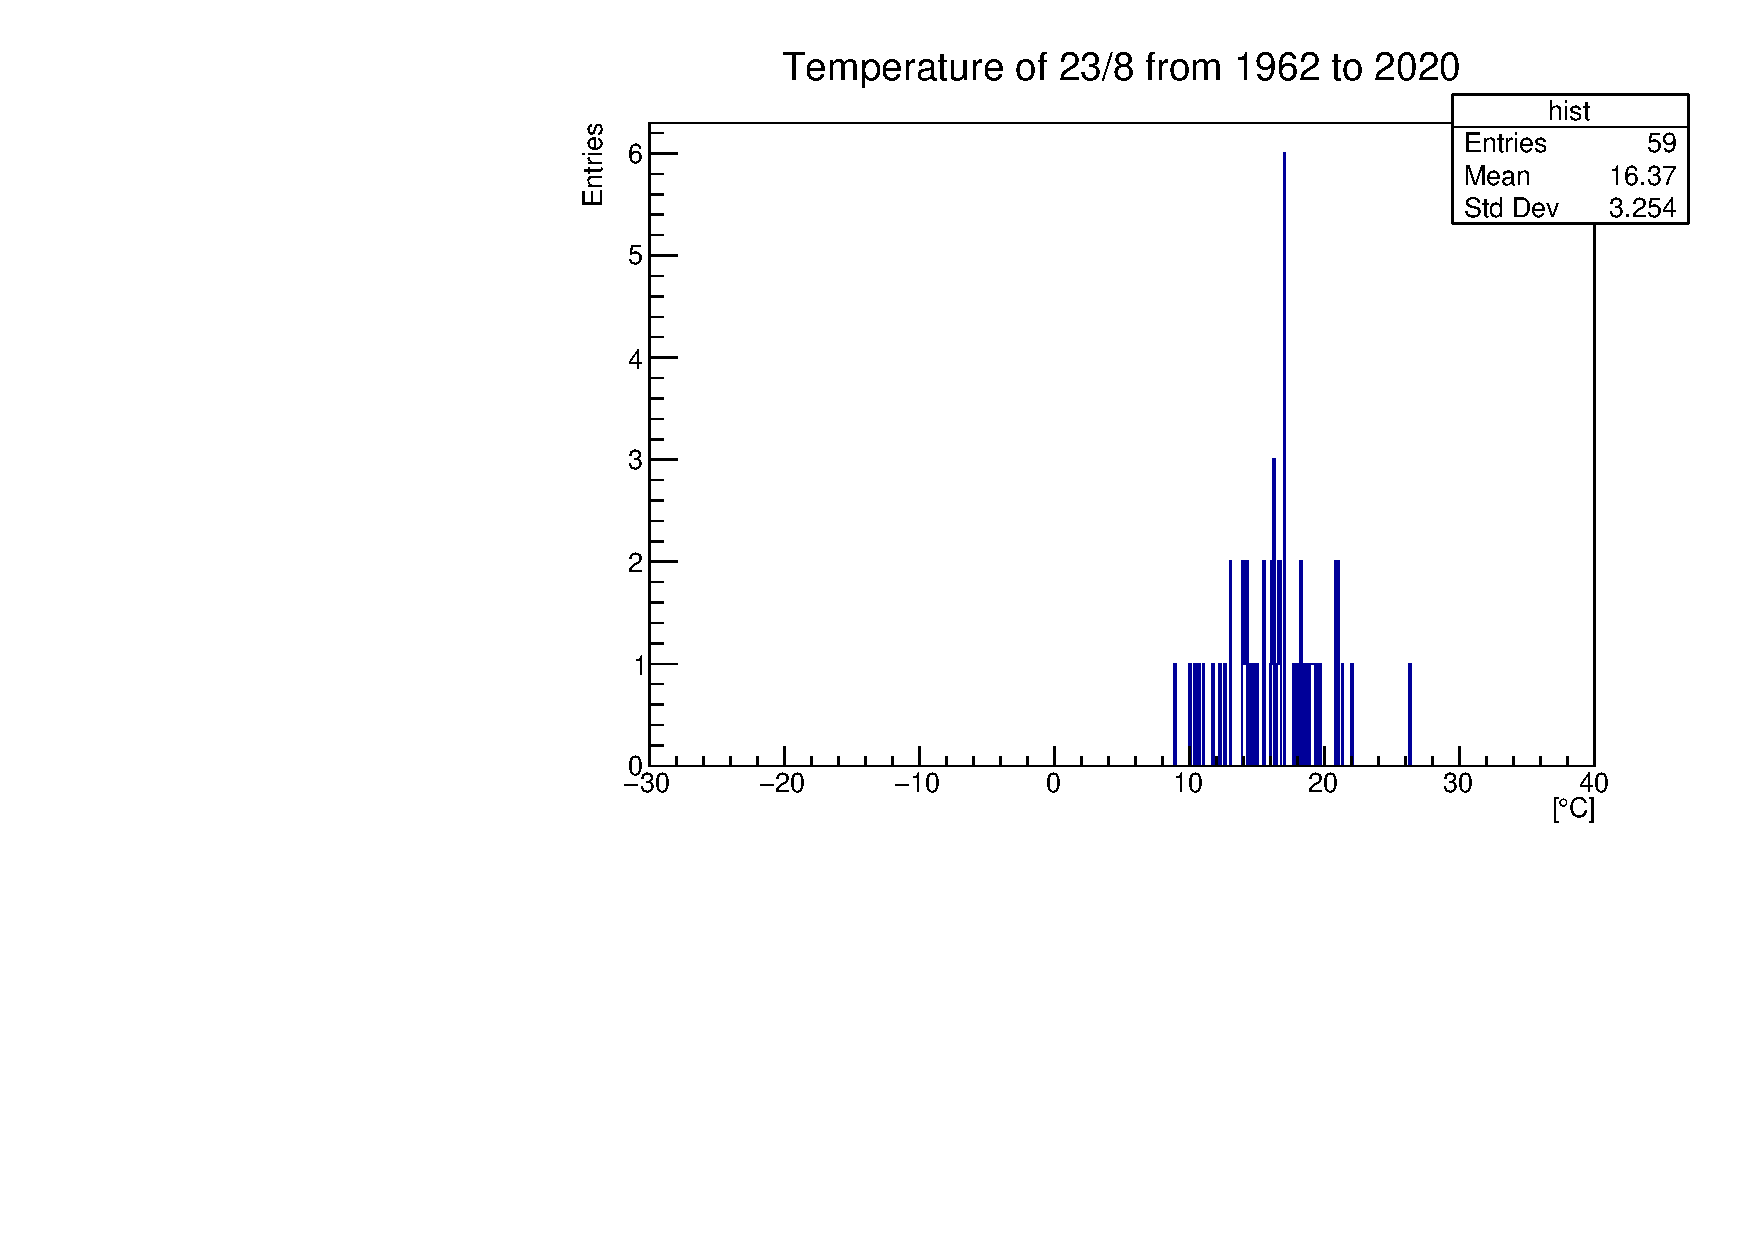
\includegraphics[scale=0.6]{chrisFig1.pdf}
\caption{Temperature of Umeå Airport in 23/8 from 1962 to 2020.}
\end{figure}


\begin{figure}[H]
\centering
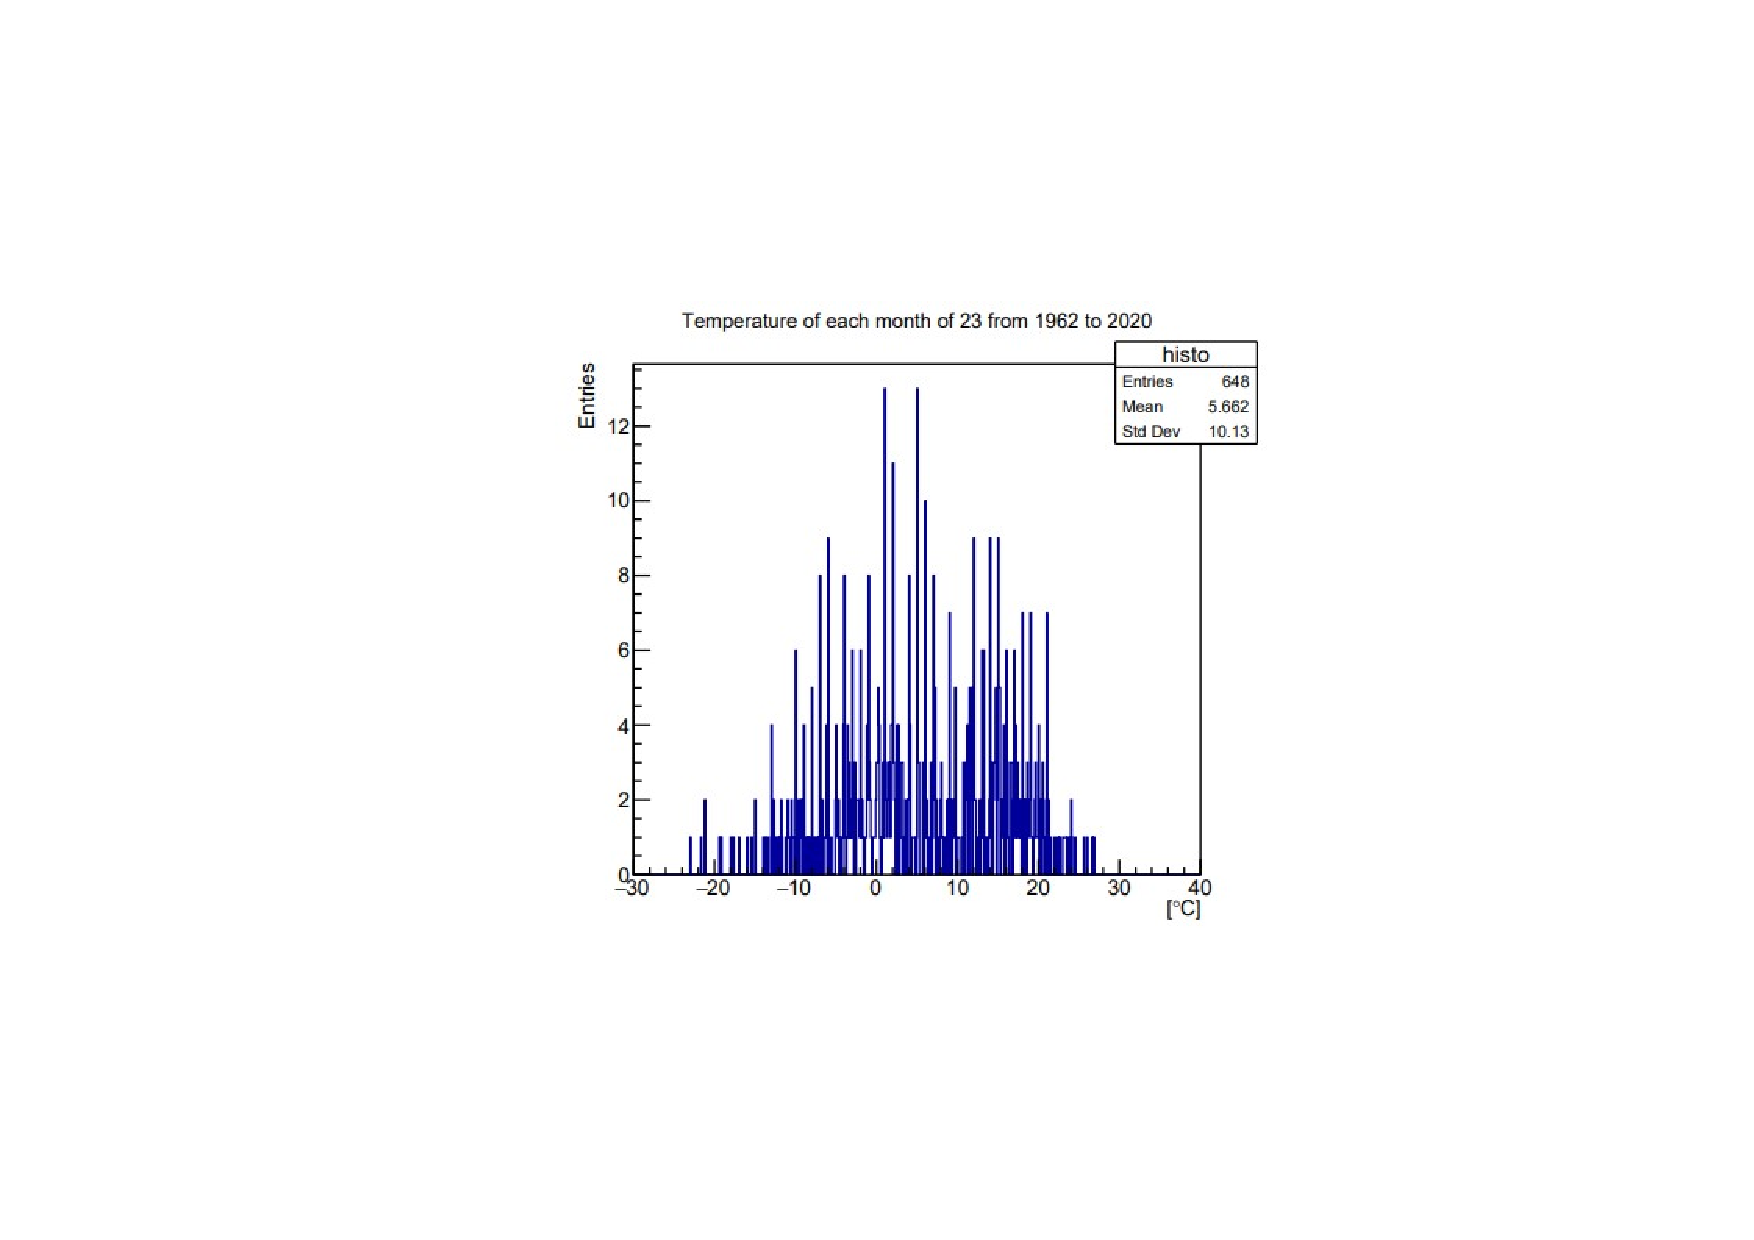
\includegraphics[scale=0.7]{chrisFig3.pdf}
\caption{ Temperature of Umeå Airport in each of the date of 23 since 1962 to 2020.}
\end{figure}




%Figure 1.1 shows the temperature for each month of 23/8 from 1962 to 2020.The mean temperature and the standard deviation is 16.37 and3.254 respectively.We can predict the probability of particular tmeperature by using the mathematical below:
%Z=(X-μ)/σ where Z=Standard score,,σ=standard deviation,μ=population mean
%For example if we want to predict what is the probability for the coming 23/8 to be in the temperature of 12°c.By applying the above equation,
%Z=(12-16.37)/3.254
%Z=-1.34
%By looking the table below(figure1.2), we can observe the probability of different value of standard score.

%In this case, the probabilty will be in0.09.

%Figure 1.2 show each of the date 23 in every month since 1962 to 2020. The mean and the standard deviation are 5.662 and 10.43 respectively.
%As discussed above, we can use the same formula to predcit the temperature of the coming date 23 for having specific temperature.

%Figure 1.1 having a lower standard deviation than figure 1.2, which means that the data in fig.1,1 are more less disperse and more closing to the mean, which lead to a more focusing graph.




\section{Discussion}
%In order to make the histogram, i have use of the excel and root. Firstly, I use the finding function in excel to locate the string or the data I need. However, it is in a string format, and i need to separate the temperature data from the string. Hence i make use of the data analysis function in excel. It can sepraate the string by detecting each of the symbol(such as ;,) in the string. As a result i can seprate the temperature data I need from the original excel file.After that I use Win Zip to transfer the revised data to Auora. For the coding part, I create a new canvas named as c1 and with the title of Temperature of Umeå FLyplats. SInce I want to show the two graphs in the same page and in parllel, so i make use of the function of Divide(2,1). After that I create a histogram named as hist with the x,y axis be [°c], and Entries respectively. And the pixels of the histogram is set to 700. Besdies, the range of x axis is from -30 to 40. Then, I try to input the data file which named as 8-23Temp.txt into the histogram by using the command ifstream infiles and infiles.open. After that i store the data in a variable named as tmp by using the command double.

\newpage
\section{References}
[1] The code in the folder "PhilipCode" available on a remote Git repository on GitHub at \href{https://github.com/fredholmP/MNXB01-FinalProject}{https://github.com/fredholmP/MNXB01-FinalProject} . \newline

\noindent [2] The code in the folders INSERT CHRIS'S FOLDERS LOCATION HERE available on a remote Git repository on GitHub at \href{https://github.com/fredholmP/MNXB01-FinalProject}{https://github.com/fredholmP/MNXB01-FinalProject} . \newline

\noindent [3] The data available from January 1st 1884 at 07.00 up until June 1st 2021 at 06.00 for the city Borås, provided by Lund Univeristy in association with the course MNXB01 during the autumn semester of 2022. At the time of writing, this data may be downloaded from the website \href{https://www.smhi.se/data/meteorologi/ladda-ner-meteorologiska-observationer}{https://www.smhi.se/data/meteorologi/ladda-ner-meteorologiska-observationer}  . \newline


\noindent [4] The data available from DAY TIME up until DAY TIME for the "Umeå Flygplats" measuring station, provided by Lund Univeristy in association with the course MNXB01 during the autumn semester of 2022. At the time of writing, this data may be downloaded from the website \href{https://www.smhi.se/data/meteorologi/ladda-ner-meteorologiska-observationer}{https://www.smhi.se/data/meteorologi/ladda-ner-meteorologiska-observationer} . 






\end{document}
